\documentclass{beamer} 
\input{xypic} 
\xyoption{color} 

%\usetheme{Singapore} 
\usetheme{CambridgeUS}
\usepackage{ bbold }

%breaksthrough proofs

\makeatletter
\newenvironment<>{proofs}[1][\proofname]{%
    \par
    \def\insertproofname{#1\@addpunct{.}}%
    \usebeamertemplate{proof begin}#2}
  {\usebeamertemplate{proof end}}
\makeatother


% expression abbreviations 
\newcommand{\hlgy}[1]{\ensuremath{H_{*}(#1)}}
\newcommand{\rhlgy}[1]{\ensuremath{\widetilde{H}_{*}(#1)}} 
\newcommand{\gk}{\ensuremath{\mathcal{G}_{k}}} 

% basic diagram commands
\newcommand{\namedright}[3]{\ensuremath{#1\stackrel{#2}
 {\longrightarrow}#3}}
\newcommand{\nameddright}[5]{\ensuremath{#1\stackrel{#2}
 {\longrightarrow}#3\stackrel{#4}{\longrightarrow}#5}}
\newcommand{\namedddright}[7]{\ensuremath{#1\stackrel{#2}
 {\longrightarrow}#3\stackrel{#4}{\longrightarrow}#5
  \stackrel{#6}{\longrightarrow}#7}}
\newtheorem{defi}{Definition}
\newtheorem{teo}{Theorem}
\newtheorem{prop}{Proposition}

\title{A topological three-dimensional quantum field theory of gravity. }  
\author{Ingrid Membrillo}
%\author{ Dr Stephen Theriault}
\date{December 2014} 

\begin{document} 



%\begin{frame}
%\titlepage
%\end{frame} 

%\begin{frame}\frametitle{Plan}
%\begin{enumerate}
%\item {Motivation and background}
%\medskip
%\item {Axiomatic formulation of a topological quantum field theory}
%\medskip
%\item {State sum invariants as a TQFT of gravity}
%\medskip
%\item {Conclusions}
%\medskip
%\item
%\end{enumerate}
%\end{frame}

%\begin{frame}\frametitle{1) Motivation and background} 

%Quantum gravity (QG) seeks to describe gravitational field through the principles of quantum mechanics. 
%\begin{figure}[H] 
%\begin{center}
%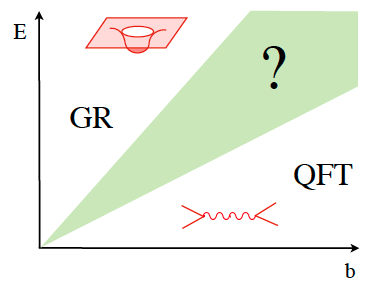
\includegraphics[width=0.35\textwidth]{QG1}
%\end{center}
%\caption{(a) $X\vee Y$; (b) $\Sigma X=S^1\wedge X$.}
%\end{figure}

%\end{frame}


%To find an adequate formulation of such a theory hasn't been an easy task. There are two big competitors at present:
%\begin{itemize}
%\medskip
%\item String theory
%\item Loop quantum gravity (Spinfoam as a covariant version)
%\end{itemize}




%\begin{frame}{1) Motivation and background}

%\medskip

%General relativity is the discovery that spacetime and the gravitational field are the same physical entity. All fields we know exhibit quantum properties at some scale, therefore it is believe spacetime to have quantum properties as well.
%\begin{figure}[H] 
%\begin{center}
%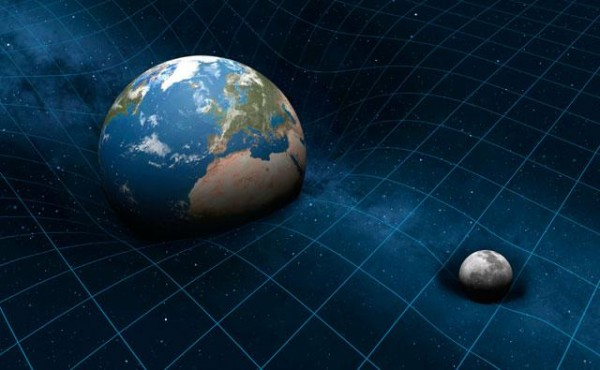
\includegraphics[width=0.7\textwidth]{gr.jpg}
%\end{center}
%\caption{(a) $X\vee Y$; (b) $\Sigma X=S^1\wedge X$.}
%\end{figure}

%\begin{itemize}
%\item With Hilbert spaces and operators (hamiltonian)
%\item As as sum over paths (lagrangian)
%\end{itemize}

%\end{frame}


%\begin{frame}\frametitle{1) Motivation and background}

%\begin{defi}
%A \emph {differential manifold} of dimension $n$ is a topological space $M$ with a family of bijective maps $\phi_\alpha:U_\alpha\subset M\rightarrow V_\alpha\subset \mathbb R^n$ such that 
%\medskip

%\begin{enumerate}[i)]
%\item $\underset{\alpha}{\bigcup}U_{\alpha}=M$
%\item for all $\alpha, \beta$ such that $U_{\alpha\beta}:=U_\alpha\cap U_\beta\neq\emptyset$, the sets $\phi_\alpha(U_{\alpha\beta})$ and $\phi_\beta(U_{\alpha\beta})$ are open in $\mathbb{R}^n$ an the maps 
%$\phi_\beta\circ\phi_{\alpha}^{-1}$ are smooths.
%\end{enumerate}
%\end{defi}
%\medskip
%\pause

%The pairs $(U_\alpha, \phi_\alpha)$ are called coordinate charts. The set of all charts is called an atlas. We will also require that any two points have disjoint neighborhoods and the atlas of $M$ is countable. 


%\end{frame} 

%\begin{frame}\frametitle{1) Motivation and background}
%\begin{defi}
%Let $M$ and $N$ be differentiable manifolds. A continuous map $f:M\rightarrow N$ is called $differentiable$ in $p$ if for every chart $(V,\phi)$ with $f(p)\in V$ there exists a chart $(U,\psi)$ with $p\in U$ such that $f(U)\subset V$ and 
%$\psi\circ f\circ\phi^{-1}$ is differentiable in $\phi(p)$.
%\end{defi}
%\pause

%\begin{defi}
%A differentiable bijective map $f:M\rightarrow N$ with $f^{-1}$ differentiable is called a \emph{diffeomorphism}.
%\end{defi}
%\end{frame}

\begin{frame}
\frametitle{ Axiomatic formulation of Topological Quantum Field Theory }
From the mathematical point of view we expect that all quantum field theories  keep
\begin{itemize}
\item general features of quantum theory (probabilistic)
\item topological framework of spacetime

\end{itemize}

Both features are embraced by the precise notion of a topological quantum field theory.
\medskip

M. Atiyah (1988) gave a formal mathematical framework to develop quantum theories in physics.
\end{frame}

\begin{frame}\frametitle{ Axiomatic formulation of Topological Quantum Field Theory}

\begin{defi}
A topological quantum field theory (TQFT) in dimension $d+1$  consist of the following data:
\medskip

Fixed an integer $d$, consider smooth oriented manifolds $M$ of dimension $d+1$ (with boundary) and also smooth closed oriented manifolds $X$ of dimension $d$. 
\pause
\medskip

\begin{itemize}
\item To each  $X$ we associate functorially \textbf{a finite-dimensional complex vector space Z}(X).  
\medskip
\pause

\item To each $M$, whose boundary is $X$ we associate a \textbf{vector Z}(M) $\in$ \textbf{Z}(X).
\end{itemize}


%A topological quantum field theory (TQFT) in dimension $d$ defined over a ground ring $R$, consist of the following data:
%\medskip
%\pause
%\begin{enumerate}[A)]
%\item A finitely generated  $R$-module $Z(\Sigma)$ associated to each oriented closed smooth $(d-1)$-dimensional manifold $\Sigma$.
%\medskip
%\pause
%\item An element $Z(M)\in Z(\partial M)$ associated to each oriented smooth $d$-dimensional manifold (with boundary) $M$.
%\end{enumerate}
\end{defi}

%$Z(M)$ is also called the \emph{partition function}.

\end{frame}


\begin{frame}\frametitle{ Axiomatic formulation of Topological Quantum Field Theory}

These data are subject to the following properties (\textbf{axioms}):
\medskip

\begin{enumerate}[1)]
\item %\textbf{Z} is functorial with respect to orientation preserving diffeomorphisms of $X$ and $M$. That is
An orientation preserving diffeormorphism $f:X\rightarrow X'$ induces an isomorphism 
\begin{equation*}
\textbf{Z} (f):\textbf{Z} (X)\rightarrow \textbf{Z}(X')
\end{equation*}
and if $g:X'\rightarrow X''$ then
\begin{equation*}
\textbf{Z} (fg)=\textbf{Z}(f)\textbf{Z} (g)
\end{equation*}
\pause

%If $f$ extends to an o. p. diff. $M\rightarrow M'$, with $\partial M=\Sigma$, $\partial M'=\Sigma'$, then $Z(f)$ take $Z(M)$ to $Z'(M)$.

\end{enumerate}
\end{frame}

\begin{frame}\frametitle{ Axiomatic formulation of Topological Quantum Field Theory}
\begin{enumerate}[2)]
\item $\textbf{Z} (X^{*})=\textbf{Z} (X)^{*}$ where $X^{*}$ is $X$ with opposite orientation and $\textbf{Z} (X)^{*}$ denotes the dual vector space. 
%Note that theres is nothing said about the orientation of $M$.
%\begin{itemize}
%\item When $R$ is a field, $Z(\Sigma)$ and $Z(\Sigma)^{*}$ are dual vector spaces.  
%\medskip 

%\item If R=$\mathbb{Z}$ the relation is like that between integer homology and cohomology
%\end{itemize}
\pause

\item [3)]\textbf{Z} is multiplicative.
\end{enumerate}
Thus, for disjoint unions
\begin{equation*}
\textbf{Z} (X_1\cup X_2)=\textbf{Z} (X_1)\otimes \textbf{Z} (X_2).
\end{equation*}

\end{frame}

\begin{frame}\frametitle{Axiomatic formulation of Topological Quantum Field Theory}
Moreover if $\partial M_1=X_1\cup X_3$, $\partial M_2=X_2\cup X_3^{*}$ and $M=M_1\cup_{X_3}M_2$ is the manifold obtained by identification of the common $X_3-component$.
\begin{figure}[H] 
\begin{center}
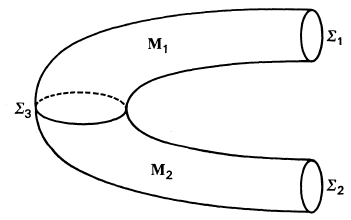
\includegraphics[width=0.4\textwidth]{bordism}
\end{center}
%\caption{(a) $X\vee Y$; (b) $\Sigma X=S^1\wedge X$.}
\end{figure}
\pause

%Then we require
%\begin{equation*}
%\textbf{Z} (M)=<\textbf{Z} (M_1),\textbf{Z} (M_2)>
%\end{equation*}
%where $<,>$ denotes the natural pairing

\begin{equation*}
Z(\Sigma_1)\otimes Z(\Sigma_3)\otimes Z(\Sigma_3)^{*}\otimes Z(\Sigma_2)\rightarrow Z(\Sigma_1)\otimes Z(\Sigma_2)
\end{equation*}

\end{frame}

\begin{frame}\frametitle{Axiomatic formulation of Topological Quantum Field Theory}

%The multiplicative axiom shows that when $X=\emptyset$ the vector space $\textbf{Z}$ is zero or isomorphic to $\mathbb{C}$. 
%\medskip
%\pause

\begin{itemize}

\item [4a)] When $X$ is the empty $d$-dimensional manifold 
\begin{equation}
\textbf{Z}(\emptyset)=\mathbb{C}.
\end{equation}
\end {itemize}
\medskip
\pause

%Similarly  when $M=\emptyset$, $Z(M)\in \mathbb{C}$ %is an idempotent element.
\begin{itemize}
\item [4b)]  Similarly, when $M= \emptyset$  
\begin{equation}
\textbf{Z}(\emptyset)=1\in\mathbb{C}
\end{equation}
\end {itemize}
\medskip
\pause
Note that when $M$ is a closed $d$-dimensional manifold so that $\partial M=\emptyset$, then
\begin{equation*}
\textbf{Z(M)}\in\textbf{Z}(\emptyset)=\mathbb C
\end{equation*}
That means, \textbf{Z(M)} is a \textbf{numerical invariant} of $M$.

\end{frame}

\begin{frame}\frametitle{State sum model as a 3D TQFT of gravity}

Einstein equations (movement equations) can be derived through minimizing the action \emph{S}:
\medskip

\begin{equation*}
S= \frac{1}{16\pi}\int R\sqrt{det(g_{\mu\nu)}}d^4x
\end{equation*}
\medskip
\pause

1961 Regge gave a discrete formulation of general relativity using triangulated manifolds. 
\begin{figure}[H] 
\begin{center}
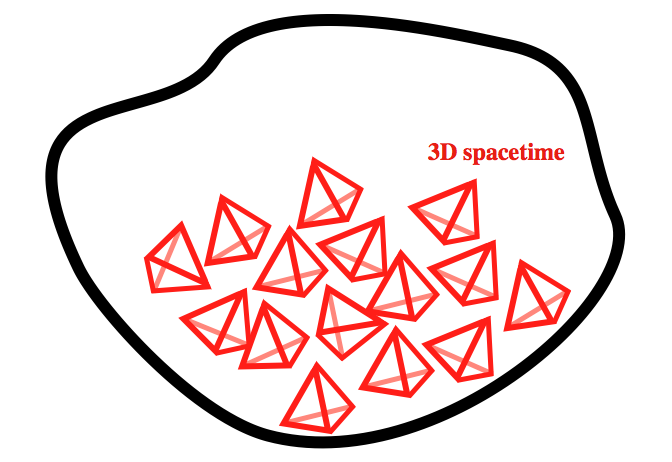
\includegraphics[width=0.35\textwidth]{regge}
\end{center}
%\caption{(a) $X\vee Y$; (b) $\Sigma X=S^1\wedge X$.}
\end{figure}

\end{frame}

\begin{frame}\frametitle{State sum model as a 3D TQFT of gravity}
Regge showed that the  curvature of a triangulated n dimensional manifold is encoded in the $(n-2)$ skeleton. 
\begin{figure}[H] 
\begin{center}
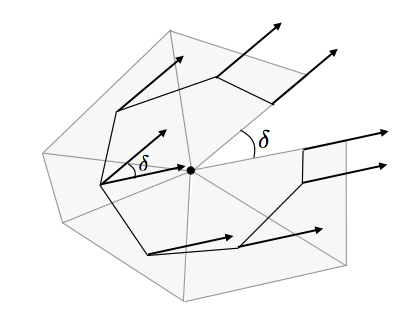
\includegraphics[width=0.35\textwidth]{pt}
\end{center}
%\caption{(a) $X\vee Y$; (b) $\Sigma X=S^1\wedge X$.}
\end{figure}


The discrete form of the action S from which Einstein field equations are derived is given by 

\begin{equation*}
S_R=\sum\left|\sigma^{i}(T)\right|\varepsilon_{i}
%S_R=\sum\frac{\partial\left|\sigma^{i}\right|}{\partial l_{j}}\varepsilon_{i}=0
\end{equation*}


\end{frame}

\begin{frame}\frametitle{State sum model as a 3D TQFT of gravity}
In quantum mechanics the action is replaced by a \textbf{partition function Z}:
\begin{equation*}
Z=\int e^{iS}D(x)
%S_R=\sum\frac{\partial\left|\sigma^{i}\right|}{\partial l_{j}}\varepsilon_{i}=0
\end{equation*}

Given a manifold M, \textbf{Z}(M) obtained from the TQFT will have the physical \textbf{meaning of the partition function}. 

\end{frame}



\begin{frame}\frametitle{State sum invariants}

In 1991 Turaev-Viro developed a 3 dimensional TQFT of gravity  called the \textbf{state sum model.} 
\begin{defi}
Given a 3 dimensional manifold and a triangulation, a \textbf{state} is an assignment of an irreducible representation of $SU(2)$ to each edge of the triangulation. This are labeled by a non-half integer parameter $\textbf{j}$.
\end{defi}

\begin{figure}[H] 
\begin{center}
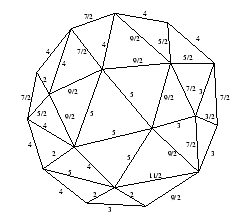
\includegraphics[width=0.3\textwidth]{surf}
\end{center}
%\caption{(a) $X\vee Y$; (b) $\Sigma X=S^1\wedge X$.}
\end{figure}

\end{frame}


\begin{frame}\frametitle{State sum invariants}

\begin{figure}[H] 
\begin{center}
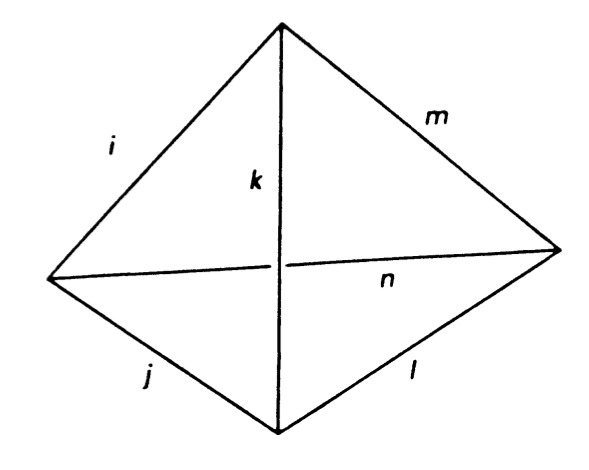
\includegraphics[width=0.25\textwidth]{tet}
\end{center}
%\caption{(a) $X\vee Y$; (b) $\Sigma X=S^1\wedge X$.}
\end{figure}
\pause

\begin{defi}
The \textbf{weight} of the state is defined by
\begin{figure}[H] 
\begin{center}
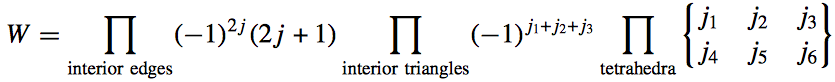
\includegraphics[width=0.7\textwidth]{ssum}
\end{center}
\end{figure}
\pause
The \textbf{state sum} (partition function) is obtained by summing over all values of the variables, subject to fixed values on the boundary.
\begin{equation*}
\textbf{Z}(M)=\Sigma W
\end{equation*}

\end{defi}
%\caption{(a) $X\vee Y$; (b) $\Sigma X=S^1\wedge X$.}


%For each triangulated closed surface F we define a $K$-module C(F) to be the module freely generated over $K$ by admissible colorings of $F$.
%If $F=\emptyset$, then we put C(F)=K.  

\end{frame}




\end{document}



